\documentclass[conference]{IEEEtran}
\IEEEoverridecommandlockouts
% The preceding line is only needed to identify funding in the first footnote. If that is unneeded, please comment it out.
\usepackage{cite}
\usepackage{amsmath,amssymb,amsfonts}
\usepackage{algorithmic}
\usepackage{graphicx}
\usepackage{textcomp}
\usepackage{xcolor}
\usepackage{subcaption}
\def\BibTeX{{\rm B\kern-.05em{\sc i\kern-.025em b}\kern-.08em
    T\kern-.1667em\lower.7ex\hbox{E}\kern-.125emX}}

\makeatletter
\def\endthebibliography{%
  \def\@noitemerr{\@latex@warning{Empty `thebibliography' environment}}%
  \endlist
}
\makeatother


\begin{document}

\title{SplitterGUI\\
{\large GUI Application of Mining Fine-Grained Sequential Patterns in Semantic Trajectories}
\thanks{The SplitterGUI project files can be downloaded at
$github.com/dzakybd/Datastream-project$}
}

\author{\IEEEauthorblockN{Tanjung Dion, Fawwaz Dzaky Zakiyal}
\IEEEauthorblockA{\textit{Department of Electrical and Computer Engineering} \\
\textit{Pusan National University}\\
Busan, Republic of Korea \\
\{tanjung.dn, dzakybd\}@gmail.com}}

\maketitle

\begin{abstract}
Semantic trajectory is a sequence of timestamped places wherein each place has information about spatial location and a semantic label. By mining fine-grained pattern that satisfy semantic consistency, spatial compactness and temporal continuity, it will give benefit such as urban planning and targeted advertising. One of the state-the-art method to mine the fine-grained pattern is Splitter algorithm. Firstly, it find set of coarse patterns and their snippets by using PrefixSpan, and then find the set of fine-grained patterns using mean shift method. In this project we build, SplitterGUI, GUI application to visualize the process of the Splitter algorithm. We also discuss the key techniques in Splitter and conduct an experiment using 4SQ database to demontrate the result of SplitterGUI.

\end{abstract}

\begin{IEEEkeywords}
fine-grained pattern, semantic trajectories, GUI application.
\end{IEEEkeywords}

\section{Introduction}
The sequential patterns can be found in a trajectory database, if it properly extracted. It become benefit for targeted advertising, urban planning, location prediction, etc. In other hand, classic sequential pattern mining algorithms cannot work effectively in semantic trajectories, a sequence of time-stamped places wherein each place has information about spatial location and a semantic label. Because of the places in the continuous space cannot be regarded as independent items, so independent place cannot be used to find the frequent sequences. Instead, semantic label need to be grouped to form frequent sequential patterns. But, there is also a challenge to get fine-grained sequential patterns, that it must fulfill requirements of spatial compactness (compact area for each place category), semantic consistency (consistent place ID in each place category) and temporal continuity (limited time constraint).
\par
The process of mining fine-grained pattern have been proposed by Zang et. al \cite{zhang2014splitter}. They provide two-step approach to obtain fine-grained sequential patterns. First-step, obtain the coarse patterns from the semantic trajectory data using the full projection method to modify PrefixSpan. The result patterns will fullfil the semantic and temporal constraints. Second-step, splitting each coarse patterns into fine-grained patterns that fulfill the spatial constraint through top-down pattern discovery process using weighted snippet shift by Epanechnikov kernel.
\par
In this project, aiming at implementing the mining fine-grained pattern method proposed by Zang et. al \cite{zhang2014splitter} and build the GUI application to visualize the process of the Splitter algorithm, called SplitterGUI. It make the database, course patterns and fine-grained patterns into a visualized map by determined Splitter algoritm's parameters. Afterwards, we discuss the key techniques in Splitter and conduct an experiment using 4SQ database to demontrate the result of SplitterGUI.


\section{Implementation}
\subsection{System Design}
\begin{figure}[!ht]
\centering
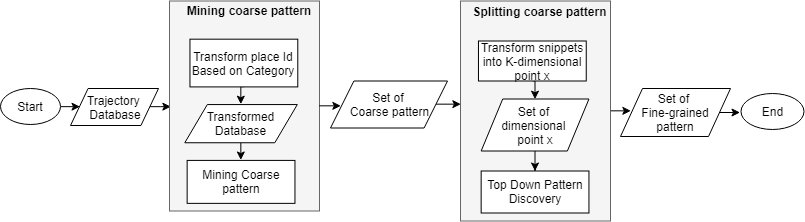
\includegraphics[width=0.55\linewidth]{splitter}
\caption{System Design}
\label{fig:systemdesign}
\end{figure}
Figure \ref{fig:systemdesign} show the process of mining fine-grained pattern in semantic trajectories. This method consist of two part: mining coarse pattern and splitting coarse pattern. Mining coarse pattern is a process to find sequential pattern that satisfy semantic consistency and temporal continuity. In the first step, we add trajectory database that have information about place id, movement time, group id, and spatial location to the system. This trajectory database will be transformed into semantic trajectory database by grouping place id based on category. However, we still keep the original place id in each category to prevent one trajectory from being counted repeatedly. By doing this process, our trajectory database will satisfy semantic consistency.
\par
Then, PrefixSpan algorithm will be used to mining the coarse pattern. In the PrefixSpan algorithm, we include all post-fixes to avoid missing pattern under the given time constrain. Output from mining coarse pattern is set of coarse pattern that will be used in the next process. The next process is finding fine-grained pattern that satisfy spatial compactness in by splitting a coarse pattern in top down manner. Set of coarse pattern from previous process will be transformed into K-dimensional point x.
\par
Then, we employ mean shift clustering to extract the dense and compact snippet cluster based on the support and variance threshold. To speed up the process, the unqualified snippet cluster will be organized into several disjoint communities. By only clustering each communities, we can gradually reduce the kernel windows in clustering method to speed up the clustering process.

\subsection{Key techniques in Splitter}
\subsubsection{Mining Coarse Pattern}
Before mining coarse pattern, trajectory database D should be transformed to semantic trajectory by grouping each place based on its category. The purpose is to find any frequent sequences that have similar categories. For example, Fig. \ref{fig:transformed-database} shows database transformation with office $=G_{1}$, shop $=G_{2}$, restaurant $=G_{3}$. 

\begin{figure}[!ht]
	\centering
	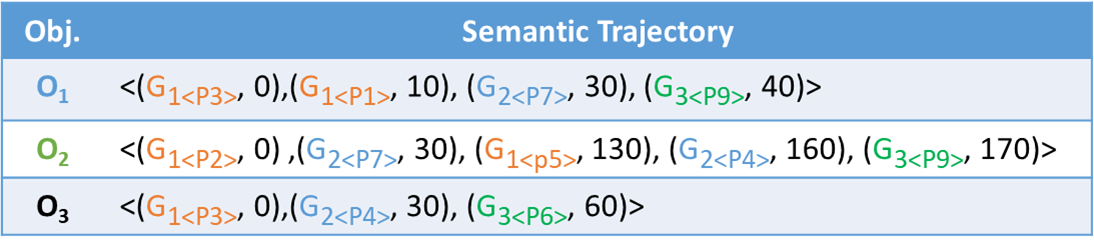
\includegraphics[width=1\linewidth]{transformed_database}
	\caption{Semantic trajectory database}
	\label{fig:transformed-database}
\end{figure}

After transformation, we mining sequential pattern that satisfy support threshold $\sigma$ and time constraint $\Delta t$ using PrefixSPan algorithm. PrefixSpan algorithm use frequent item as short pattern and prefixes to build projected database then grow the short pattern by searching local frequent item in projected database. However, PrefixSpan algorithm should be modified to satisfy our coarse pattern. \ref{fig:mining-coarse-pattern} shows the modified prefix span algorithm. First, we extract all frequent item at least $\sigma$ in semantic trajectory D. Then for each item we build item-projected database as S using full projection. Full projection means that we extract all pattern that occurred in database. For example, object 0 in \ref{fig:transformed-database} has 2 pattern $P_{3}\rightarrow P_{7}\rightarrow P_{9}$ and $P_{1}\rightarrow P_{7}\rightarrow P_{9}$.
\par
Output this item as our short pattern and then grow this pattern by calling PrefixSpan function. This function has similar procedure with initial projection function. However, we check time constraint when searching frequent item in projected database. We also call this PrefixSpan function recursively to grow the pattern until the pattern cannot be grown anymore. Output of this algorithm is list of coarse pattern with its snippet (i.e. $P_{1}\rightarrow P_{7}\rightarrow P_{9}$), group (i.e. $G_{1}\rightarrow G_{2}\rightarrow G_{3}$), and pattern length (i.e. 3).  

\begin{figure}[!ht]
	\centering
	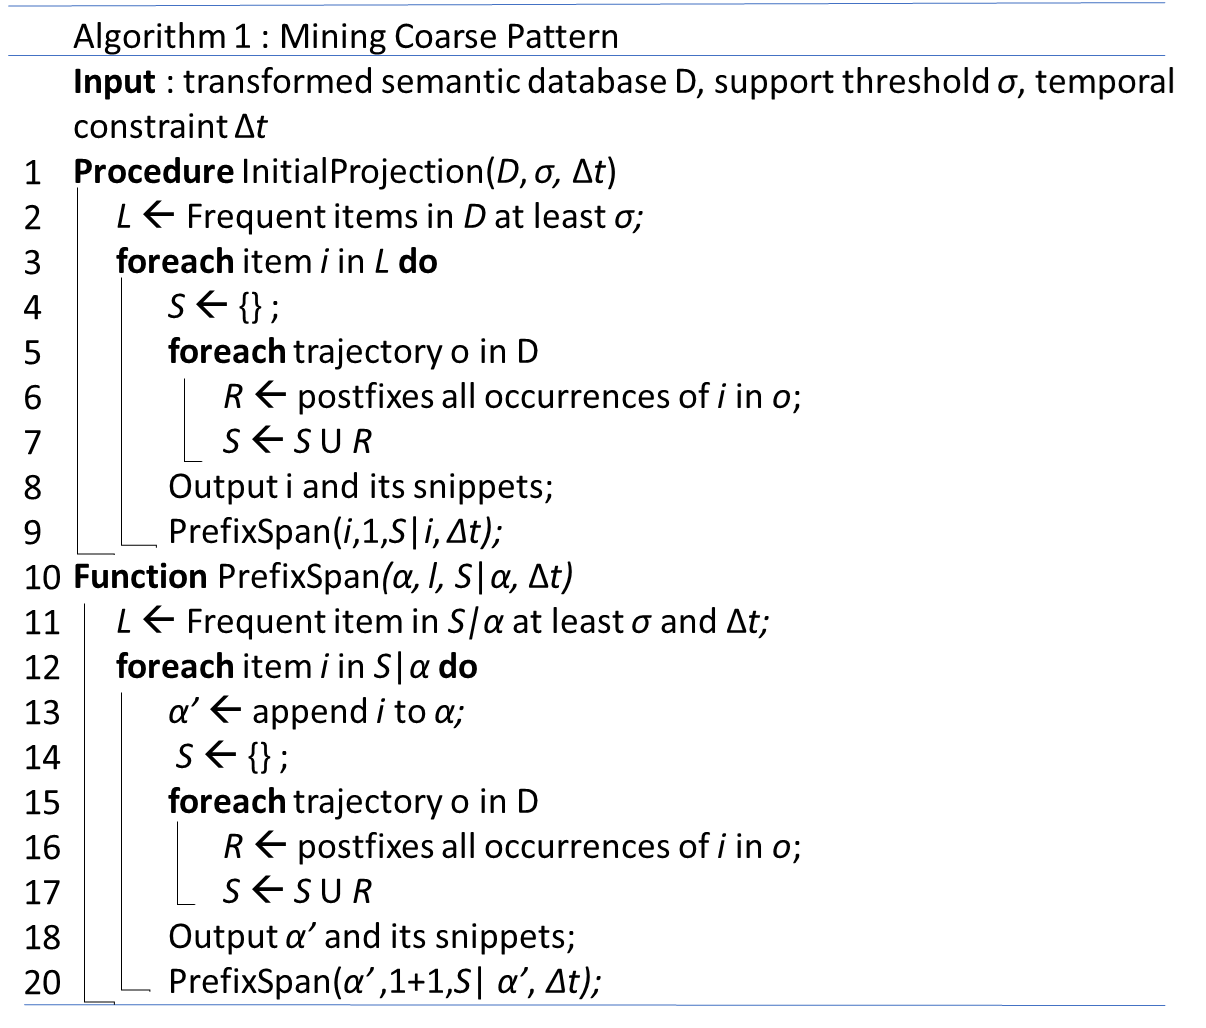
\includegraphics[width=1.0\linewidth]{mining_coarse_pattern}
	\caption{Mining coarse pattern algorithm \cite{zhang2014splitter}}
	\label{fig:mining-coarse-pattern}
\end{figure}

\subsubsection{Finding Fine-Grained Pattern}
The result of coarse pattern has satisfy support threshold $\sigma$ and time constraint $\Delta t$. Next step is checking the spatial variance of place in each group category. For example, graph representation of coarse pattern is shown in Fig. \ref{fig:graph-coarse-pattern}. Spatial location of place $P_{5}$ with other place in group $G_{1}$ is to far. Therefore, we have to prune pattern $P_{5}\rightarrow P_{4}\rightarrow P_{6}$ from fine-grained pattern. 

\begin{figure}[!h]
	\centering
	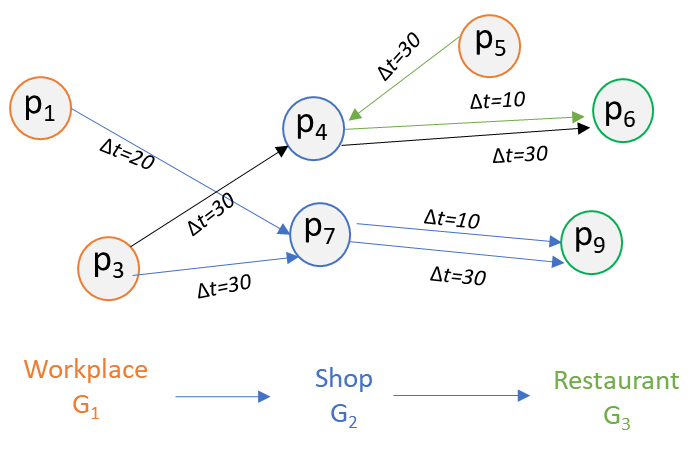
\includegraphics[width=1\linewidth]{graph_coarse_pattern}
	\caption{Graph representation of coarse pattern result}
	\label{fig:graph-coarse-pattern}
\end{figure}

For finding fine-grained pattern, mean shift clustering algorithm is used because it does not need any prior knowledge and only use one parameter called bandwidth. Bandwidth parameter is used to limit the area of clustering. The main idea of mean shift algorithm is choosing random point as the center and use bandwidth to limit the coverage area of clustering. Then calculate mean shift vector to shift the center point toward new point that more dense than previous point. For windows kernel, we use Epanechnikov kernel. 
\par
Before clustering, we transform snippet in each coarse pattern into a 2k-dimensional point x by assembling the coordinates of each snippet. Then, the number of visitors is added to x as weight. Algorithm 2 shows how to cluster point using mean shift algorithm. Output of this algorithm is set of cluster.

\begin{figure}[h!]
	\centering
	\includegraphics[width=1.0\linewidth]{"algorithm weighted snippet"}
	\caption{Weighted snippet shift algorithm \cite{zhang2014splitter}}
	\label{fig:algorithm-weighted-snippet}
\end{figure}
Specify the best bandwidth size is not an easy task. If bandwidth is small, there will be many small snippet cluster that not exceed support threshold $\sigma$. On the other hand, large bandwidth make the large cluster that cannot satisfy variance threshold $rho$. Therefore, we have to start with large bandwidth then dampen it until no more pattern exist. For this problem, notion of $\gamma$-community is presented to reduce the cost of repeating the process in large cluster. $\gamma$-community can be defined as connected component between two cluster. Two cluster can be connected if distance between two cluster no more than $\gamma$.  Fig. \ref{fig:lamda-community} shows the example of $\gamma$-community. 
\begin{figure}[!h]
	\centering
	\begin{subfigure}[b]{0.4\linewidth}
		\includegraphics[width=\linewidth]{"cluster example"}
		\caption{Snippet cluster}
	\end{subfigure}
	\begin{subfigure}[b]{0.4\linewidth}
		\includegraphics[width=\linewidth]{"lamda community"}
		\caption{$\gamma$-community}
	\end{subfigure}
	\caption{Example of $\gamma$-community}
	\label{fig:lamda-community}
\end{figure}

Algorithm 3 shows refine coarse pattern algorithm. First, we cluster snippet using weighted snippet shift with bandwidth h. For each cluster we check if the support is at least $sigma$ and the variance is no more than $rho$ then report as fine grained pattern and remove from cluster set. Set $\gamma$ as root 2 multiply by dampening factor and current bandwidth. Then construct set of $\gamma$-community from cluster S that are not reported as fine grained pattern. For each $\gamma$-community, check if the support is at least $sigma$ then repeat the process of refine coarse pattern algorithm. 

\begin{figure}[!h]
	\centering
	\includegraphics[width=1\linewidth]{"refine coarse"}
	\caption{Refine coarse pattern algorithm \cite{zhang2014splitter}}
	\label{fig:refine-coarse}
\end{figure}

\section{Demonstration}

\subsection{Database}
This project will use the real database, 4SQ that collected from Foursquare check-in sequence in New York. It consists of 48564 places that divided into 417 place with list of categories and it stored semantic trajectories from 14909 users. 4SQ database provides 3 files:
\begin{enumerate}
\item \textit{Sequences}, it contains users semantic trajectories including attributes of check-in time-stamp and place ID.
\item \textit{Places}, it contains information about the places (place ID, latitude, longitude, list of category ID).
\item \textit{Category}, it contains information of place category ID corresponding with its place category name.
\end{enumerate}

\subsection{Implementation detail}
We will re-implement the process of mining fine-grained pattern using Java programing language. For improving GUI performance, we use G4P library (http://www.lagers.org.uk/g4p/) that based on OpenGL and JavaFX rendering engines. The other purpose is to support geographical map visualization from unfolding library (http://unfoldingmaps.org/) that also use OpenGL rendering engines. We also using other libraries such as apache commons (http://commons.apache.org) to support our program. 
\par 
Input of our program is database file that will be used to build graph representation as our database in the system. This graph representation is based on adjacency list that is shown in \ref{fig:adjacency}. There are 4 object: database, trajectory, place, and category. Database object has list of trajectory that have id to represent people and have list of sequence to represent the movement. Each movement is a list of timestamped place that has information of place id, position, and category. In the next step, we implement mining coarse pattern algorithm and refine coarse pattern algorithm for finding fine-grained pattern from the database. 
\begin{figure}[!h]
	\centering
	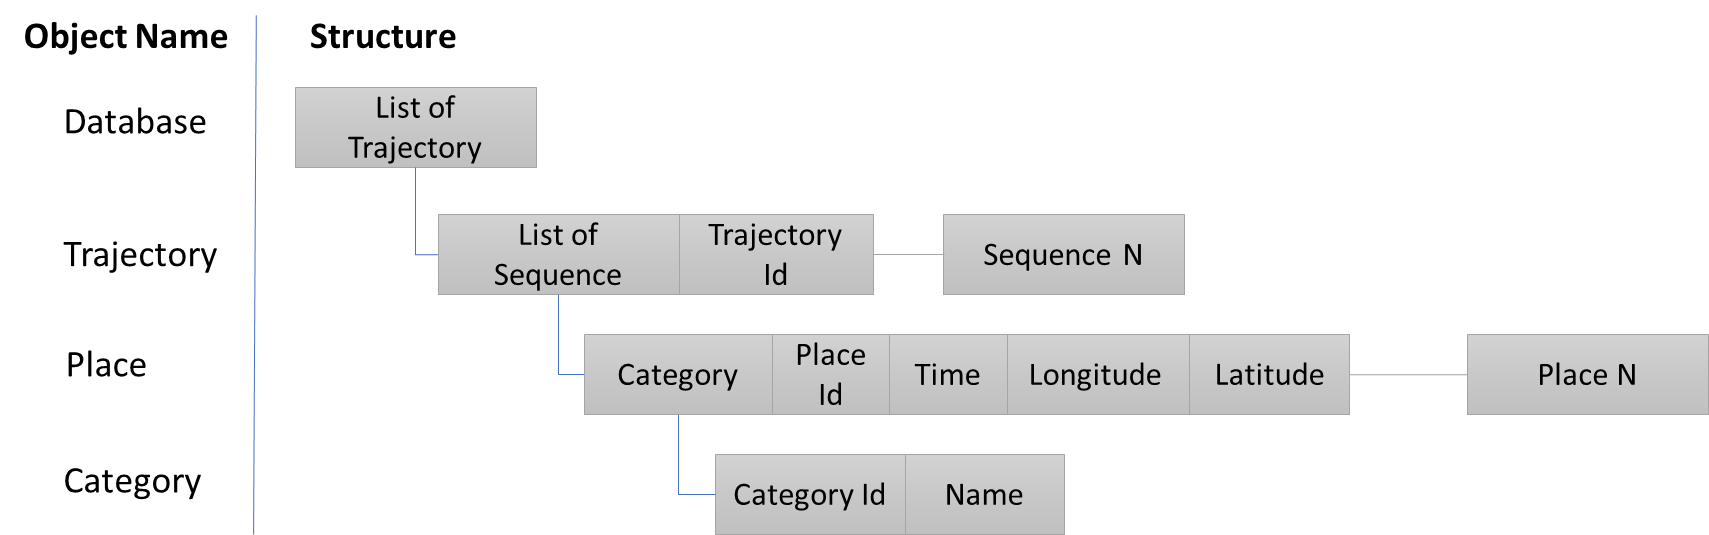
\includegraphics[width=1\linewidth]{adjacency}
	\caption{Structure of database in adjacency list representation}
	\label{fig:adjacency}
\end{figure}

The user interface of program will be provided as shown in the Fig. \ref{fig:visual}. The figure shows the illustration of our program. There are 3 database input in .csv format for category and place and .txt format for the sequence data. There are also 6 input parameters in the configuration field. Support threshold, pattern length, and time limit for mining coarse pattern, and variance threshold, dampening factor for refine the coarse pattern. In the first step, we have to create the database. After that,we can mine coarse pattern first then perform refine coarse pattern or do both coarse pattern and refine coarse pattern respectively.
\begin{figure}[!h]
	\centering
	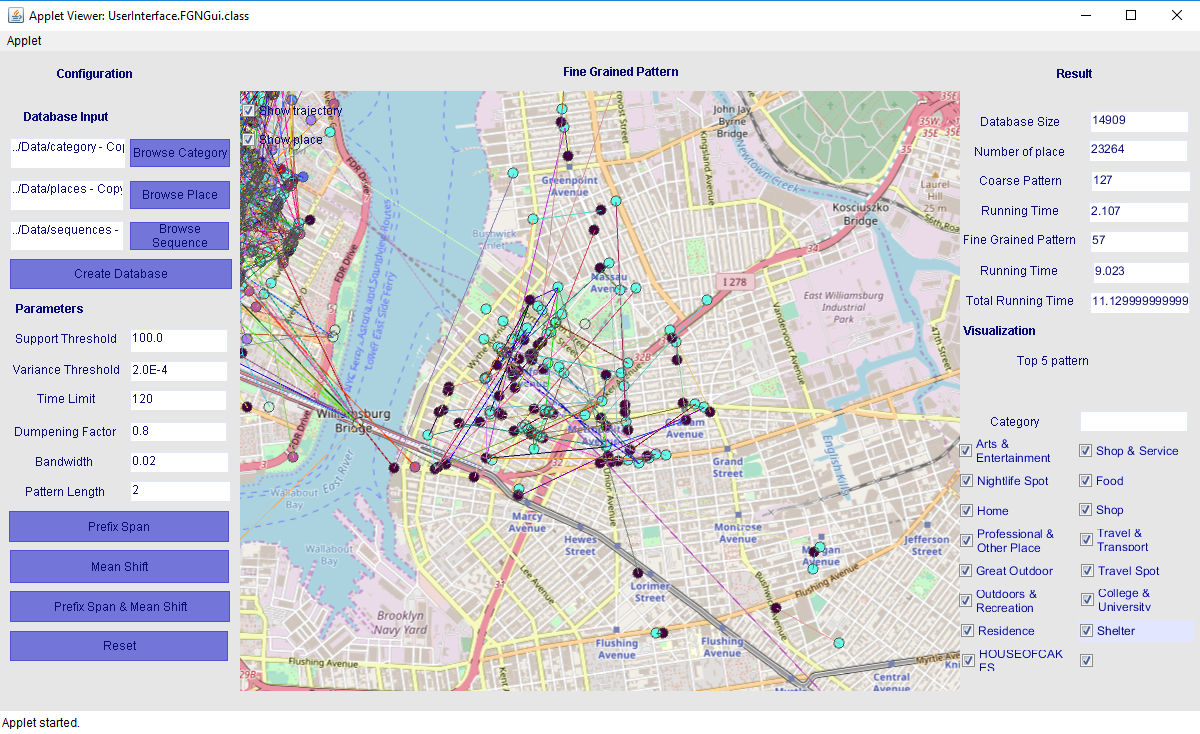
\includegraphics[width=1\linewidth]{visual}
	\caption{Visualization}
	\label{fig:visual}
\end{figure}

\subsection{Experiment}
Experiment is conducted in windows 10 Pro 64-bit running on Processor Intel Core I5 7500 @3.40GHz, 4GB of RAM, and Intel HD Graphics 630. First, we choose database file and fill the input parameters support threshold 100, variance threshold 0.0004, time constraint 120, dampening factor 0.8, Bandwidth 0.02, and minimum pattern length 2. In this application, minimum pattern length is used to set the minimum length of pattern when mining coarse pattern. Secondly, We create the database by pushing create database button. Before, pushing the button, we decided to unchecked show trajectory radio button because it decrease the performance when creating line marker in map visualization. In this function, it also search the number of category that exist in the database. From 48.564 of distinct places, we get 15 categories. Fig. \ref{fig:mapdatabase} shows the original number of place in the database.   

\begin{figure}[h!]
	\centering
	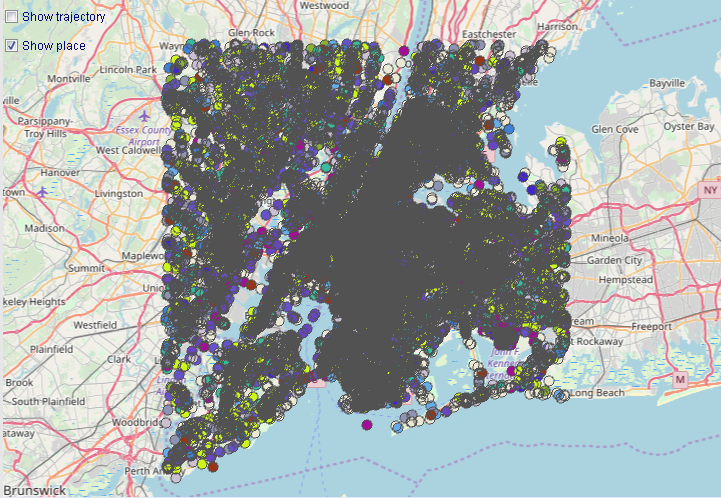
\includegraphics[width=1\linewidth]{mapDatabase}
	\caption{Visualization of place found in from database}
	\label{fig:mapdatabase}
\end{figure}

After creating database, we run prefix span algorithm for mining coarse pattern. In this process, places that occurs in the coarse pattern is 23264. It means that the process reduce places up to half of number of place occurred in the original database. The running time of mining coarse pattern is 3.685 seconds. Therefore, prefixspan algorithm is fast enough to finding a pattern in a database. Coarse pattern found from the database is 127 which consist of pattern length of 2 (109 patterns) and pattern length of 3 (18 patterns). The highest support or the total number of trajectory that using this pattern in the length of 2 is shop $\rightarrow$ food which contains 2905 of trajectories. For the pattern length of 3, the highest support is food $\rightarrow$ shop $\rightarrow$ food which used by 299 of trajectories. From this result we can assume that a lot of people like to go the food area then go shopping then go to the another food area. Fig. \ref{fig:mapcoarse} shows place reduction after mining coarse pattern.

\begin{figure}[h!]
	\centering
	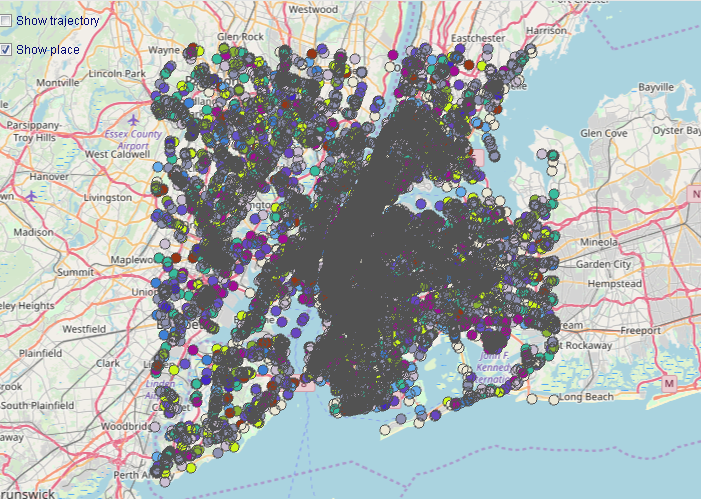
\includegraphics[width=1\linewidth]{mapCoarse}
	\caption{Visualization of place found after mining coarse pattern}
	\label{fig:mapcoarse}
\end{figure}

The next step is refine coarse pattern to get fine grained pattern from the database. After we push mean shift button in the left side, the system will begin to refine coarse pattern. Fine grained pattern found in the database using the inputed parameter are 57 patterns. Using the inputed parameters, we cannot find fine-grained pattern that have length 3 occurred in the coarse pattern. It means that our coarse pattern that have length 3 is not satisfy the spatial closeness based on the parameters. Most trajectory follows pattern shop $\rightarrow$ food that have support 1063. Fig \ref{fig:maprefine} shows that places are clustered in a dense location only.    
\begin{figure}[h!]
	\centering
	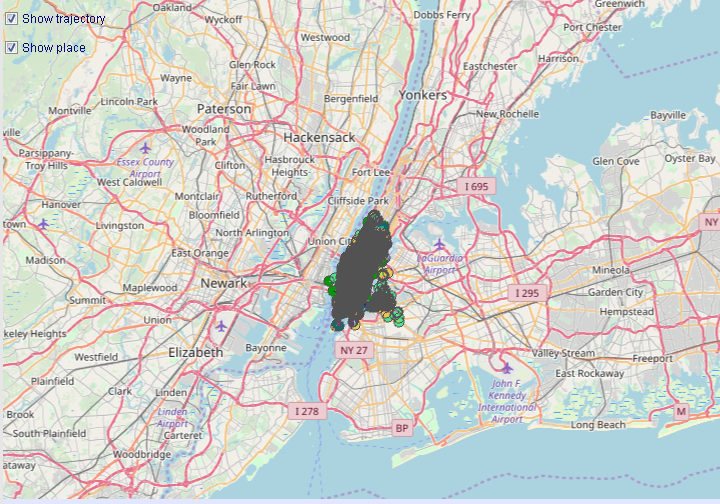
\includegraphics[width=1\linewidth]{mapRefine}
	\caption{Visualization of place found after mining coarse pattern}
	\label{fig:maprefine}
\end{figure}

\section{Conclusions}
After doing the implementation of splitter: Mining Fine-Grained Pattern, it shows that it capable to find pattern that are frequent, in limited time movement, and have spatial closeness. In this paper, it also shown that the running time of splitter to find fine-grained pattern only take total running time below 20seconds from database that consist of 14909 trajectory and 48564 of places. In the first step, mining coarse pattern algorithm is used to searching pattern that satisfy support threshold $\sigma$ and time constraint $\Delta$t. In the next step, coarse pattern will be used as the input in refining pattern that satisfy spatial variance.   



\section*{Acknowledgment}
This paper is submitted to fulfill term project task from Stream Database class (Fall 2018), Pusan National University.

\bibliographystyle{IEEEtran}
\bibliography{refs}

\end{document}
